\documentclass[letterpaper]{article}
\usepackage[letterpaper,top=1in,bottom=1in,left=1in,right=1in]{geometry}
\usepackage[utf8]{inputenc}
\usepackage{graphicx}
\usepackage[T1]{fontenc}
\usepackage{times}      % Loads the Times-Roman Fonts
\usepackage{mathptmx}   % Loads the Times-Roman Math Fonts
\usepackage{helvet}
\usepackage[sf,bf]{titlesec}
\usepackage{lineno}
\usepackage{setspace}
\usepackage[style=nejm]{biblatex}
\addbibresource{references.bib}
\usepackage{caption}
\captionsetup[figure]{labelfont={sf,bf}}

\setlength{\parindent}{0em}
\setlength{\parskip}{1em}

\begin{document}

\section*{Robustness of phylogenetic analysis for detecting clusters of new HIV infections}

August Guang$^1$, Mark Howison$^2$, Mia Coetzer$^3$, Lauren Ledingham$^3$, Matt D'Antuono$^3$,
Philip A. Chan$^3$, Charles Lawrence$^4$, Casey W. Dunn$^5$, Rami Kantor$^3$

$^1$ Computing and Information Services, Brown University, Providence, RI, USA

$^2$ Research Improving People's Lives, Providence, RI, USA

$^3$ Division of Infectious Diseases, The Alpert Medical School, Brown University, Providence, RI, USA

$^4$ Division of Applied Mathematics, Brown University, Providence, RI, USA

$^5$ Department of Ecology and Evolutionary Biology, Yale University, New Haven, CT, USA

\doublespace
\linenumbers
\section*{Abstract}

\textbf{Background:} Phylogenetic analysis of HIV sequences obtained as part of clinical care is increasingly applied to detect clustering of new HIV infections and inform public health interventions to disrupt transmission. Conventional approaches summarize the within-host HIV diversity with a single consensus sequence per individual of only the \emph{pol} gene, obtained from Sanger or next-generation sequencing (NGS).

\textbf{Methods:} We evaluate the robustness of the consensus approach and the potential benefits of considering the within-host diversity in phylogenetic analysis and cluster inference for all newly HIV-diagnosed individuals in the first half of 2013 at the largest HIV center in Rhode Island, USA. We compare Sanger and NGS-derived \emph{pol} and near-whole genome consensus sequences to an alternate approach that samples many sequences per individual from a profile hidden Markov model of their NGS data.

\textbf{Results:} The space of phylogenies inferred through sampling is multi-modal, suggesting that a consensus-inferred phylogeny is not an appropriate summary of within-host variation. Cluster inference differs in phylogenies from consensus sequences from Sanger and NGS data, and across gene regions.

\textbf{Discussion:} The choice of sequencing and summarization methods affects the detection of clusters, and should be considered carefully in public health applications of phylogenetic analysis to disrupt HIV transmission.

\section*{Background}

Clinicians are generally interested in inferring transmission links between HIV-infected individuals to improve HIV treatment and prevention. In the absence of reliable patient contact histories, phylogenetic analysis of viral sequence data can be used to infer transmission clusters \parencite{leitner}, under the assumption that two individuals sharing a most recent common ancestor in a phylogeny are more likely to share a transmission link in the real, unobservable transmission network. The application of phylogenetic analysis and cluster inference techniques in public health interventions to disrupt transmission was delineated as one of the four key pillars for achieving the Department of Health and Human Services' recently-announced plan for ending the HIV epidemic in the US \parencite{fauci}.

While historically the phylogenetic informativeness of the \emph{pol} region of the HIV genome was initially contested \parencite{hue, sturmer}, its use is now widespread in phylogenetic analysis and cluster inference, often due to the availability of \emph{pol} sequences from routine clinical genotyping by commercial Sanger sequencing. In a recent meta study, Novitsky \emph{et al.} (forthcoming) found that 102 out of 107 published studies of HIV cluster inference between 2016 and 2019 used the \emph{pol} region alone.

The increasing availability of NGS technology has led to longer and deeper sequencing of HIV, and data sets that cover nearly the whole genome with thousands or more reads at each site. Recent evidence suggests improvements in both phylogenetic analysis and cluster inference from near-whole genome HIV sequences obtained with NGS. For example, Yebra \emph{et al.} \parencite{yebra} found that the accuracy of phylogenetic reconstruction and cluster inference on simulated sequences improved with longer genomic regions (with the best accuracy from a gag-pol-env concatenation). Novitsky \emph{et al.} \parencite{novitsky} similarly studied the effects on cluster inference of using longer genomic regions from real near-whole genome Sanger sequences, and found that the proportion of sequences in clusters increased with longer sequence regions.

Most phylogenetic methods require a single fully resolved sequence for each individual included in the phylogeny. Accordingly, researchers often summarize the within-host variation present in NGS data sets with a consensus sequence. In the larger context of phylogenetic methods (e.g. beyond their application to HIV sequences), this consensus approach carries an underlying statistical assumption of \emph{low relative entropy} \parencite{guang}. In the context of HIV, tihs assumption is that the consensus sequence adequately captures the relevant information about the distribution of sequences that might be constructed given the within-host variation measured in deep sequencing through NGS. Some previous studies of HIV transmission dynamics have accounted for this variation with coalescent within-host evolutionary models \parencite{giardina, romero-severson}, but such models still assume a consensus sequence as the observed data.

In this study, we examine how well this assumption underlying the consensus approach holds on a data set comprising all newly HIV-diagnosed individual in the first six months of 2013 from the largest HIV center in Rhode Island, USA. We present a new analysis method called \emph{profile sampling} that uses the within-host variation in the NGS data to assess the robustness of the consensus approach for phylogenetic analysis and cluster inference.

\section*{Methods}

\subsection*{Data collection and sequencing}

Our study and data collection were approved by Lifespan's Institutional Review Board. We collected viral sequences from 37 individuals newly diagnosed with HIV during 2013 and treated at The Miriam Hospital Immunology Center in Providence, Rhode Island, USA. Inclusion criteria were: (i) HIV-infected adults, 18 years of age or older; (ii) diagnosed with HIV during the first six months of 2013; and (iii) available \emph{pol} sequence from routine drug resistance testing. Patient identifiers were removed and all analysis was conducted with de-identified sequence data.

We obtained near-whole genome viral sequences for the 37 participants using both Sanger and NGS sequencing methods. Blood specimens were obtained from participants with their consent and processed to isolate peripheral blood mononuclear cells (PMBC), buffy coats, and plasma. From the collected plasma, total nucleic acid was extracted for genotyping. An in-house genotyping assay was used to generate the near-whole genome based on previously published methods \parencite{nadai, di_giallonardo}. For each sample, two cDNA templates were generated by SuperscriptIII First Strand Synthesis System (Thermofisher, Carlsbad, CA), followed by eight separate nested PCR reactions; these eight amplicons span the near-whole genome of HIV.  Final amplicon products were sequenced by the Sanger method using 3100 Genetic Analyzer (Applied Biosystems, Foster City, CA) and sequenced by NGS using Nextera XT DNA Library Prep chemistry (Illumina, San Diego, CA) to generate multiplexed libraries for Illumina's MiSeq platform with 250 base paired-end reads. Sanger consensus sequences were generated manually using Sequencher version 5.2.4 (Gene Codes, Ann Arbor, MI) to confirm degenerate nucleotides. NGS data were processed and demultiplexed using BaseSpace cloud based application? (Illumina, San Diego, CA).

\subsection*{Profile sampling}

We introduce a new approach for incorporating within-host variation into phylogentic analysis, called \emph{profile sampling}. We start by aligning each individual's NGS reads using the hivmmer pipeline \parencite{howison}, which we extended to support near-whole genome HIV data and to perform codon-aware alignment within each gene (pending release as hivmmer version 0.3.0). Briefly, hivmmer performs quality control and error correction in overlapping regions of the read pairs using PEAR version 0.9.11 \parencite{zhang}, translates them into each possible reading frame, aligns them in amino acid space to all group M reference sequences from the Los Alamos National Lab HIV Database with the probabilistic multiple sequence aligner HMMER version 3.1b2 \parencite{eddy}, and produces a codon frequency table across the near-whole HIV genome, which we refer to as the individual's HIV \emph{profile}.

We construct fully-resolved sequences by sampling codons at each site in the genome using the codon frequencies from the profile. The collection of sampled sequences captures the empirical distribution of within-host variation at the codon level. We sample 500 sequences from each individual's profile, then collate the sampled sequences into 500 profile-sampled data sets, each having one sampled sequence per individual. We perform phylogenetic inference on each of the 500 profile-sampled data sets by estimating a multiple sequence alignment with mafft version 7.313 \parencite{katoh} and a maximum-likelihood phylogeny with the GTRCAT model and 100 rapid bootstrap replicates using RAxML version 8.2.12 \parencite{stamatakis}. In addition to the 500 profile-sampled phylogenies, we infer two additional phylogenies from the NGS consensus sequences and Sanger consensus sequences. We perform cluster inference on these phylogenies using Cluster Picker \parencite{ragonnet-cronin} with thresholds of 80\% bootstrap support and 4.5\% genetic distance. Analysis source code is available from \url{https://github.com/kantorlab/hiv-profile-sampling}.

In addition to performing these analyses on the near-whole genome sequences (``wgs''), we also perform them on subsets of the sequences in three clinicially relevant regions: the protease and reverse transcriptase regions at the beginning of the \emph{pol} gene (``prrt''), the \emph{int} gene, and the \emph{env} gene. The prrt region and \emph{int} are routinely sequenced in clinical care to detect drug resistance mutations and inform clinical choices of anti-retroviral therapy. The \emph{env} region is... Rami, why is this routinely sequenced??

\section*{Results}

\subsection*{Profile sampling captures within-host diversity}

We examine how much 

Profile sampling allows us to visualize the degree of polymorphism within a patient (Figure 1) and sample genomic sequences in proportion to the within-host variation. It can also build a consensus sequence for easy comparison of new approaches to established methods. By visualizing the degree of polymorphism, we can assess whether genomic variation exists at significantly high enough frequencies such that neither consensus genomes nor any other point estimator are sufficient summaries.

Figure 1 shows substantial variation exists in the HIV profiles of all patients. Across	all patients, we found that 5.63 percent of sites in the HIV genome are polymorphic, with 11.4 percent of those sites in the gag region, 21.4 percent of those sites in the pol region, and 29.5 percent of those sites in the env region of the genome. Here we define polymorphism to mean that a particular site has greater than 1% variation. This falls within the range of prior studies on within-host variation \parencite{li, zanini}. This suggests that consensus genomes, and in particular Sanger sequencing of the pol region, discards variation that is informative for inferring the phylogeny.

\subsection*{Phylogenetic estimates are sensitive to inter-host diversity}

Given that previous studies on individuals infected with HIV have shown high intra-patient variation, and given that we found similar results in our set of data (Figure 1), we investigated its impact on downstream topological variation in the phylogenetic tree.  The results show that trees inferred from the profile-sampled sequences do not cluster around any of the trees inferred from a genome point estimate (Figure 2).

When and MDS plot is generated for only the profile-sampled trees (Figure 3), they appeared to form two clusters. This is likely due to zoom on the profile-sampled trees, as can be seen from the axes scales for Figure 2 and Figure 3. Supertrees of the two clusters reveal that most of the clades in the two subtrees are the same, with only patients out of 37 having a different topological placement on the two trees (Figure 4). This suggests that distinct clusters of phylogenetic trees exist given the intra-patient variation, but that the differences between them are not large.  However, the consensus genome appears to be an inadequate estimate summary for the intra-patient variation, as can be seen in Figure 5.

\subsection*{Inferred clusters differ by sequencing method and genomic region}


\section*{Discussion}

A limitation of our study is the small number of participants. The participants do have a dense temporal sampling, and comprise all newly HIV-diagnosed individuals in a six month period at the largest HIV center in Rhode Island, USA, who met the inclusion criteria. However, the overall size of the HIV epidemic in Rhode Island is much larger, estimated as 2,396 individuals in 2016 \parencite{ridoh}. In future work, we hope to apply the profile sampling method to larger NGS data sets, to assess if cluster inference from Sanger versus NGS data agrees or differs especially for clusters larger than three individuals, which was the largest cluster size in our current data set.

Our construction of HIV profiles from NGS data is limited by the accuracy of the NGS assays themselves. The codon frequencies in the profiles may be biased measures of the true within-host diversity because of biases in PCR amplification during sample preparation. Sequencing protocols such as Primer ID \cite{jabara} have been introduced to reduce and correct for these biases. Unfortunately, the Primer ID protocol supports only a limited region of the HIV genome, and has not yet been extended to support near-whole genome sequencing of HIV, but future work could study this limited region to determine if cluster inference changes with the implementation of a Primer ID protocol.

The true HIV transmission network is unknown, but phylogenetic analysis and cluster inference are promising tools for aiding clinicians and public health officials \cite{fauci}. Current phylogenetic approaches do not fully utilize the information on within-host diversity available from deeper and longer NGS sequencing technologies. As NGS data sets are increasingly available and more fully sample from the current HIV epidemic, 

\printbibliography

\begin{figure}[p!]
	\caption{Intra-patient genetic diversity (defined as the average percent difference across all pairwise comparisons of the 500 profile-sampled nucleotide sequences for a patient) is highest in the env region for most individuals, and lies within the range of previously reported values.}
	\centering
	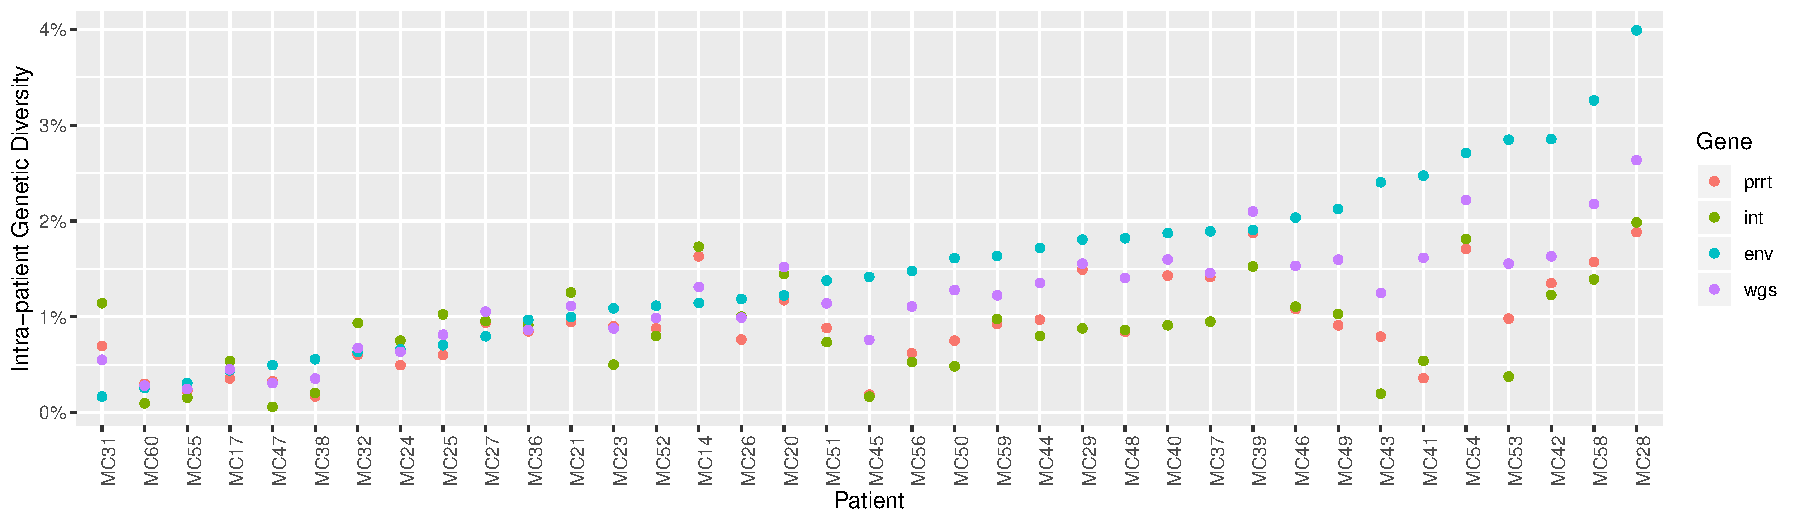
\includegraphics[width=\linewidth]{Figure1}
	\label{fig1}
\end{figure}

\begin{figure}[p!]
	\caption{Multi-dimensional scaling of pairwise geodesic distance among maximum-likelihood phylogenies from the profile-sampling approach show that the space of phylogenies inferred for the prrt and int regions are multi-modal. The phylogenies from consensus sequences (black dots) are point estimates that do not capture the full variation in phylogenies that can be inferred from deeply-sequenced NGS data.}
	\centering
	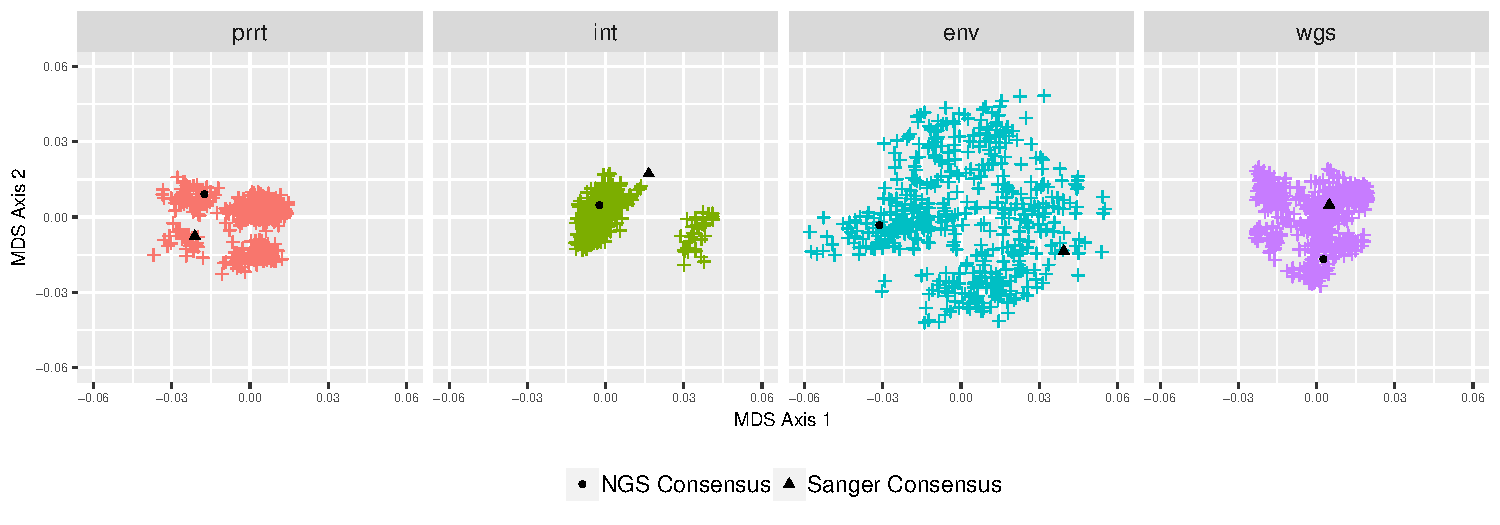
\includegraphics[width=\linewidth]{Figure2}
	\label{fig2}
\end{figure}
	
\begin{figure}[p!]
	\caption{The total branch length in each of the profile-sampled phylogenies also varies. The phylogenies from consensus sequences (black dots) can lie at extreme values within these distribution, both when considering the lengths across all branches and the lengths across only the branches at the tips.}
	\centering
	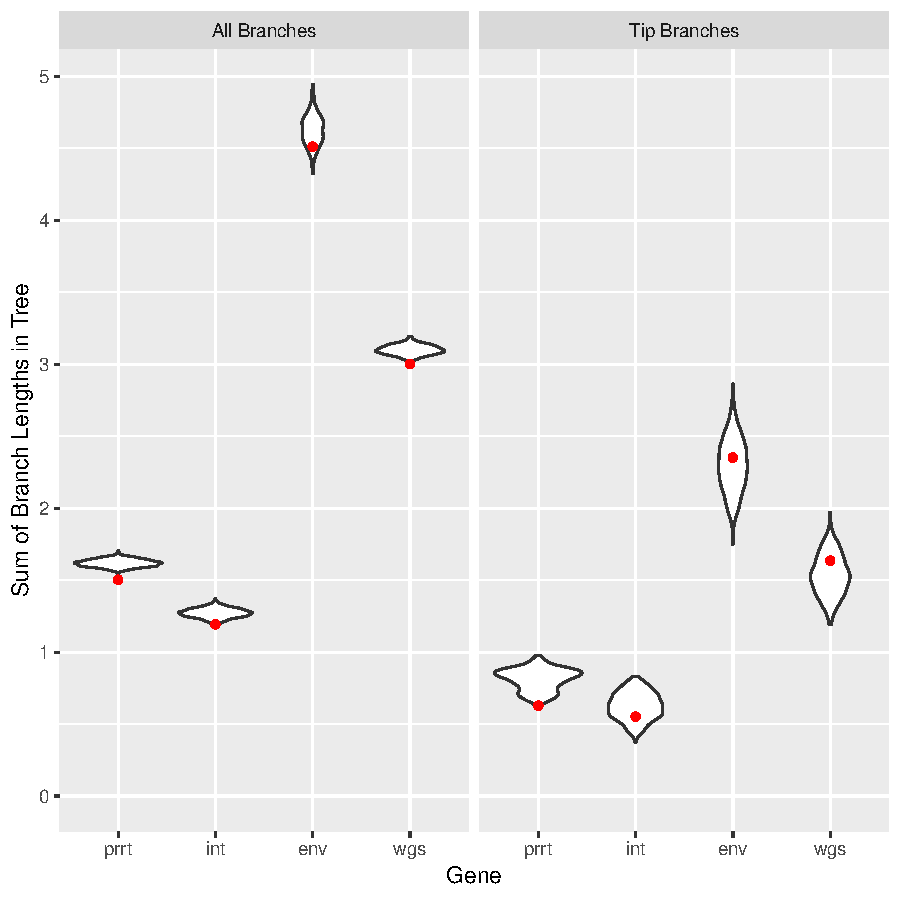
\includegraphics[width=4in]{Figure3}
	\label{fig3}
\end{figure}

\begin{figure}[p!]
	\caption{Clusters (vertical colored bars) inferred from the phylogenies of NGS consensus sequences differ across genomic regions. The largest number of clusters was inferred from the int region, and the smallest number from the env region. Profile sampling provides a bootstrapped measure of cluster support (annotation to bars).}
	\centering
	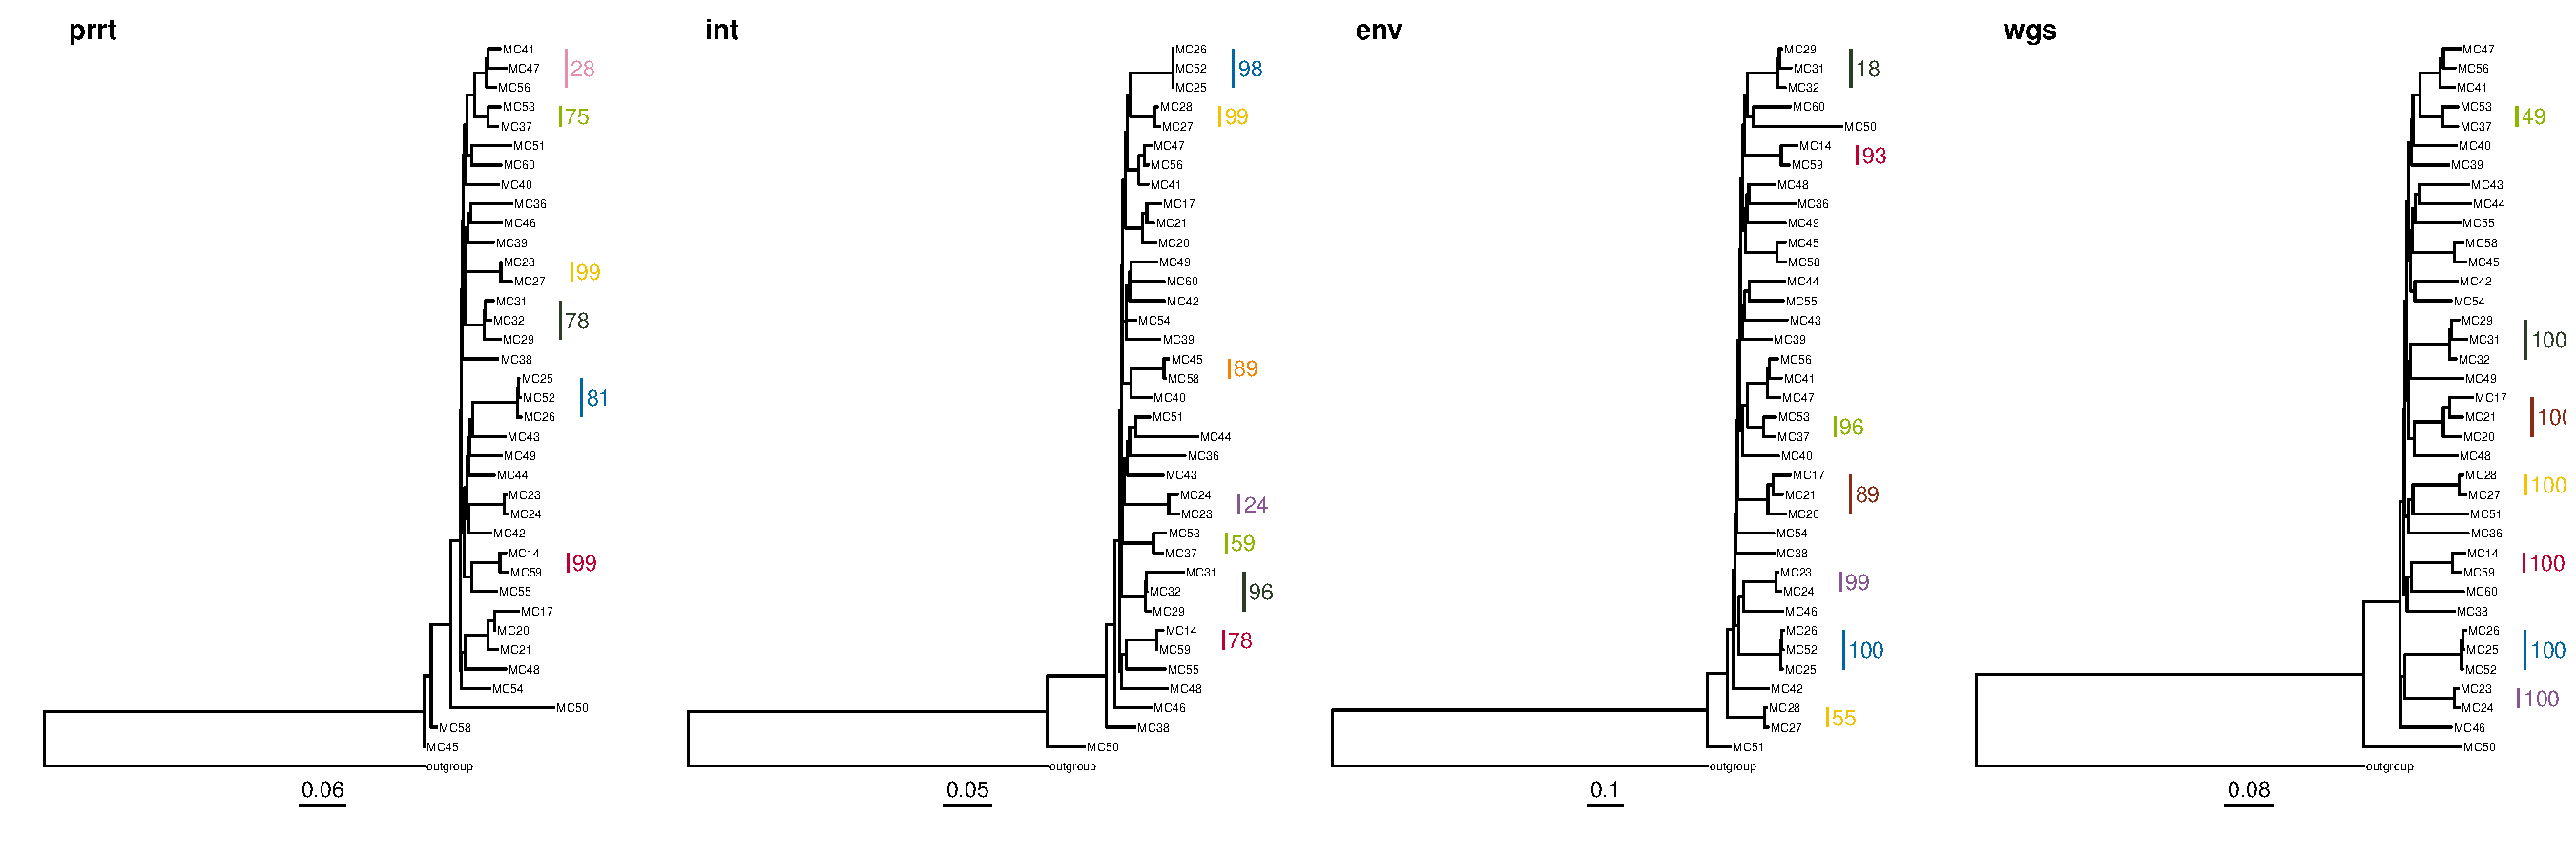
\includegraphics[width=\linewidth]{Figure4}
	\label{fig4}
\end{figure}

%\begin{figure}[p!]
%	\caption{Clusters (vertical colored bars) inferred from the phylogenies of Sanger consensus sequences differ across genomic regions. The largest number of clusters was inferred from the int region, and the smallest number from the env region. Profile sampling provides a bootstrapped measure of cluster support (annotation to bars).}
%	\centering
%	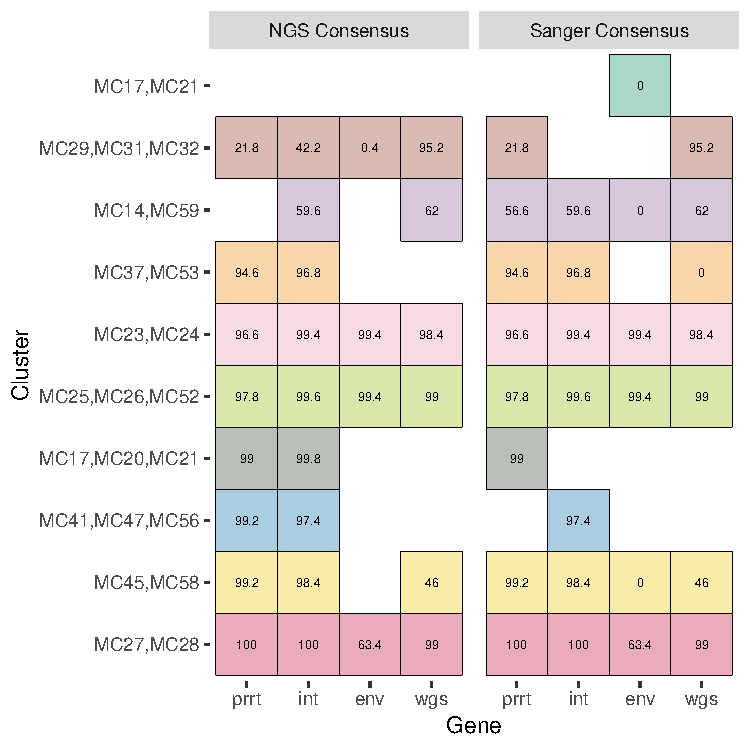
\includegraphics{Figure5}
%	\label{fig5}
%\end{figure}
%
%\newpage

\begin{figure}[p!]
	\caption{Summary of clusters identified by Sanger versus NGS consensus sequences across genomic regions. Numeric values indicate bootstrapped cluster support from the profile sampling method.}
	\centering
	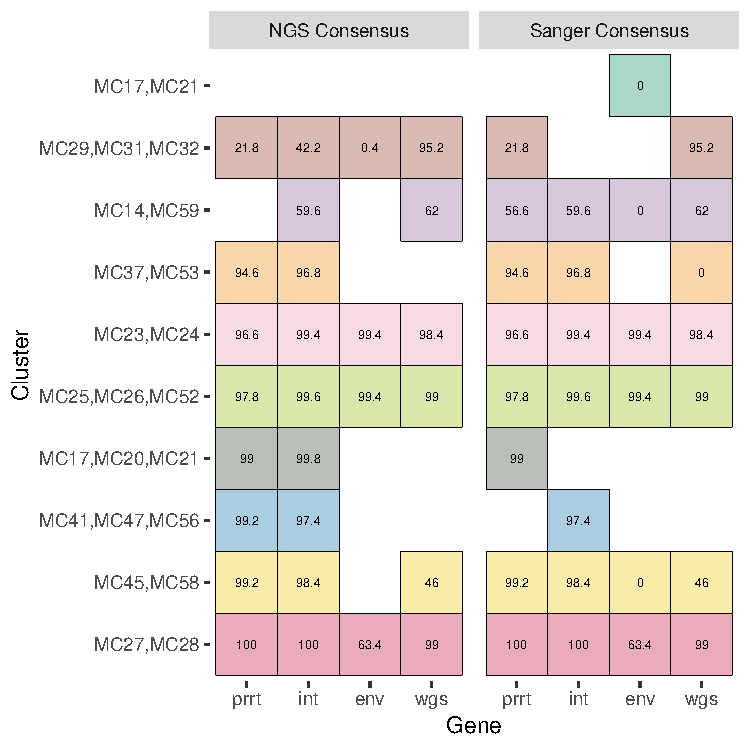
\includegraphics[width=4in]{Figure5}
	\label{fig5}
\end{figure}

\end{document}
